\documentclass[10pt]{article}

\usepackage[margin=0.75in]{geometry}
\usepackage{amsmath,amsthm,amssymb,bm}
\usepackage{xcolor}
\usepackage{cancel}
\usepackage{graphicx}
\usepackage{changepage}
\usepackage{circuitikz}
\usepackage{pgfplots}
\usepackage{physics}
\usepackage{hyperref}
\usepackage{siunitx}
\usepackage{fontspec}
\usepackage{relsize}
\usepackage{subfig}
\usepackage{todonotes}
\usepackage{multicol, multirow, booktabs}
\usepackage[breakable]{tcolorbox}
\usepackage[inline]{enumitem}

\theoremstyle{definition}
\newtheorem{problem}{Problem}
\newtheorem{soln}{Solution}

\pgfplotsset{compat=newest}
\usetikzlibrary{lindenmayersystems}
\usetikzlibrary{arrows}
\usetikzlibrary{calc}
\usetikzlibrary{positioning, fit}
\usetikzlibrary{3d, perspective}

\definecolor{incolor}{HTML}{303F9F}
\definecolor{outcolor}{HTML}{D84315}
\definecolor{cellborder}{HTML}{CFCFCF}
\definecolor{cellbackground}{HTML}{F7F7F7}
\newcommand{\ui}{\hat{i}}
\newcommand{\uj}{\hat{j}}
\newcommand{\uk}{\hat{k}}
\newcommand{\ux}{\hat{x}}
\newcommand{\uy}{\hat{y}}
\newcommand{\uz}{\hat{z}}
\newcommand{\uv}[1]{\hat{\bv{{#1}}}}
\newcommand{\pr}[1]{{#1}^\prime}
\pgfdeclarelayer{background}  
\pgfsetlayers{background,main}
\AtBeginDocument{\RenewCommandCopy\qty\SI}
\newcommand{\justif}[2]{&{#1}&\text{#2}}

\makeatletter
\newcommand{\boxspacing}{\kern\kvtcb@left@rule\kern\kvtcb@boxsep}
\makeatother
\newcommand{\prompt}[4]{
    \ttfamily\llap{{\color{#2}[#3]:\hspace{3pt}#4}}\vspace{-\baselineskip}
}

\newcommand{\thevenin}[2]{
  \begin{center}
    \begin{circuitikz} \draw
      (0,0) -- (2,0) to[battery1, l_=$V_{Th}\eq#1$] (2,2) 
      to[resistor, l_=$R_{Th}\eq#2$] (0,2)
      ;
      \draw [o-] (-.07,2.079);
      \draw [o-] (-.07,0.079);
    \end{circuitikz}
  \end{center}
}

\newcommand{\norton}[2]{
  \begin{center}
    \begin{circuitikz} \draw
      (0,0) -- (3,0) to[american current source, l_=$I_{N}\eq#1$] (3,2) -- (0,2) (2,0)
      to[resistor, l=$R_{N}\eq#2$] (2,2)
      ;
      \draw [o-] (-.07,2.079);
      \draw [o-] (-.07,0.079);
    \end{circuitikz}
  \end{center}
}

\DeclareMathOperator{\Div}{div}
\DeclareMathOperator{\Curl}{curl}

\DeclareSIUnit\mile{m}

\newcommand{\highlight}[1]{\colorbox{yellow}{$\displaystyle #1$}}

\newcommand{\ti}[1]{\widetilde{#1}}

\newcommand{\bv}[1]{\bm{\mathrm{#1}}}

\title{Physics 3130H: Assignment II}
\author{Jeremy Favro (0805980) \\ Trent University, Peterborough, ON, Canada}
\date{\today}

\begin{document}
\maketitle

% PROBLEM 1
\begin{problem}~
\begin{enumerate}[label=(\roman*)]
  \item Calculate the centrifugal acceleration due to Earth's rotation on a particle on the surface of Earth at the equator.
  \item Compute the centrifugal acceleration due to the motion of Earth about the Sun.
  \item Compare these two values and discuss why one is greater than the other.
\end{enumerate}
\end{problem}
\begin{soln}~
  \begin{enumerate}[label=(\roman*)]
    \item If we assume that the Earth is rotating such that the vector pointing from its axis of rotation to the equator forms a right angle with
          the axis, then we obtain
          \begin{align*}
            \bv{a}_c & =-\bv{\omega}\cross(\bv{\omega}\cross\bv{r})                              \\
                     & =-\omega\uz\cross(-\omega r\ux)                                           \\
                     & =\omega^2r=\frac{v_t^2}{r}\approx \qty{0.0332}{\meter\per\second\squared}
          \end{align*}
    \item Again making the right-angle approximation and assume Earth's orbit is circular we arrive at the same formula though with different values.
          We obtain a centrifugal acceleration of something on the surface of the Earth to be approximately $\qty{0.006}{\meter\per\second\squared}$.
    \item The centrifugal acceleration due to the Earth's rotation is significantly larger because the Earth's rotational velocity is significantly larger compared
          to its radius than the Earth's orbital velocity and it's orbital distance.
  \end{enumerate}
\end{soln}
\newpage

% PROBLEM 2
\begin{problem}
If a projectile is fired due east from a point on the surface of Earth at a northern latitude $\lambda$ with
a velocity $v_0$ and at an angle of inclination to the horizontal of $\alpha$, show that the lateral deflection
when the projectile strikes Earth is given by
$$d=\frac{4v_0^3}{g^2}\omega\sin\lambda\sin^2\alpha\cos\alpha,$$ where $\omega$ is the rotation frequency of Earth.
\end{problem}
\begin{soln}
  It was (and still kind of isn't) intuitive to me \emph{why} there is any Coriolis ``force'' on an eastward moving object other than the one
  which ``pushes'' its point of impact to the west due to the rotation of the Earth. I found this physics stack exchange post helpful in understanding what is happening.
  \url{https://physics.stackexchange.com/questions/43124/is-there-an-intuitive-explanation-for-the-southward-force-caused-by-the-coriolis}. Here we define the following coordinate system which we will reuse
  throughout the assignment:
  \begin{center}
    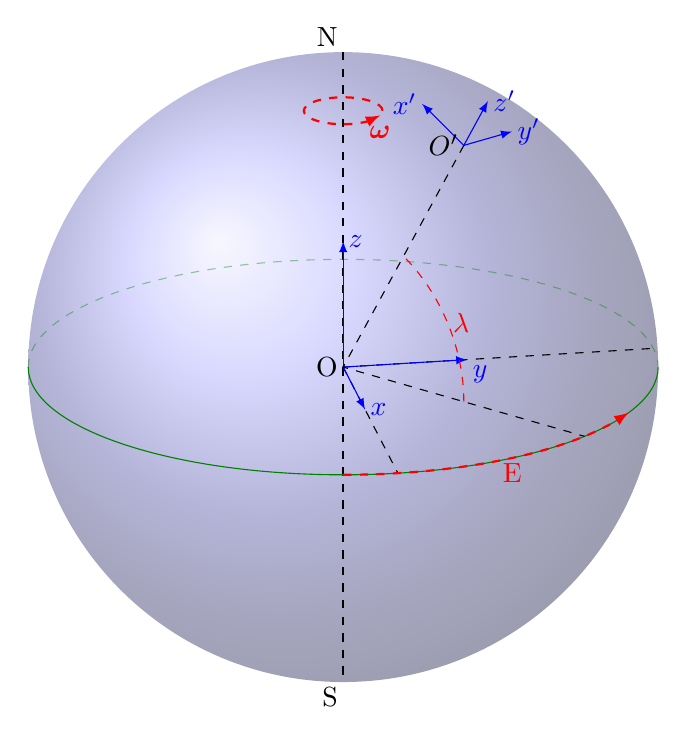
\begin{tikzpicture} % "THE GLOBE" showcase
      \newcommand\pgfmathsinandcos[3]{%
        \pgfmathsetmacro#1{sin(#3)}%
        \pgfmathsetmacro#2{cos(#3)}%
      }
      \newcommand\LongitudePlane[3][current plane]{%
        \pgfmathsinandcos\sinEl\cosEl{#2} % elevation
        \pgfmathsinandcos\sint\cost{#3} % azimuth
        \tikzset{#1/.style={cm={\cost,\sint*\sinEl,0,\cosEl,(0,0)}}}
      }

      \newcommand\LatitudePlane[3][current plane]{%
        \pgfmathsinandcos\sinEl\cosEl{#2} % elevation
        \pgfmathsinandcos\sint\cost{#3} % latitude
        \pgfmathsetmacro\yshift{\RadiusSphere*\cosEl*\sint}
        \tikzset{#1/.style={cm={\cost,0,0,\cost*\sinEl,(0,\yshift)}}} %
      }
      \newcommand\NewLatitudePlane[4][current plane]{%
        \pgfmathsinandcos\sinEl\cosEl{#3} % elevation
        \pgfmathsinandcos\sint\cost{#4} % latitude
        \pgfmathsetmacro\yshift{#2*\cosEl*\sint}
        \tikzset{#1/.style={cm={\cost,0,0,\cost*\sinEl,(0,\yshift)}}} %
      }
      \newcommand\DrawLongitudeCircle[2][1]{
        \LongitudePlane{\angEl}{#2}
        \tikzset{current plane/.prefix style={scale=#1}}
        % angle of "visibility"
        \pgfmathsetmacro\angVis{atan(sin(#2)*cos(\angEl)/sin(\angEl))} %
        \draw[current plane] (\angVis:1) arc (\angVis:\angVis+180:1);
        \draw[current plane,opacity=0.4] (\angVis-180:1) arc (\angVis-180:\angVis:1);
      }
      \newcommand\DrawLongitudeArc[4][black]{
        \LongitudePlane{\angEl}{#2}
        \tikzset{current plane/.prefix style={scale=1}}
        \pgfmathsetmacro\angVis{atan(sin(#2)*cos(\angEl)/sin(\angEl))} %
        \pgfmathsetmacro\angA{mod(max(\angVis,#3),360)} %
        \pgfmathsetmacro\angB{mod(min(\angVis+180,#4),360} %
        \draw[current plane,#1,opacity=0.4] (#3:\RadiusSphere) arc (#3:#4:\RadiusSphere);
        \draw[current plane,#1]  (\angA:\RadiusSphere) arc (\angA:\angB:\RadiusSphere);
      }%
      \newcommand\DrawLatitudeCircle[2][1]{
        \LatitudePlane{\angEl}{#2}
        \tikzset{current plane/.prefix style={scale=#1}}
        \pgfmathsetmacro\sinVis{sin(#2)/cos(#2)*sin(\angEl)/cos(\angEl)}
        % angle of "visibility"
        \pgfmathsetmacro\angVis{asin(min(1,max(\sinVis,-1)))}
        \draw[current plane] (\angVis:1) arc (\angVis:-\angVis-180:1);
        \draw[current plane,opacity=0.4,dashed] (180-\angVis:1) arc (180-\angVis:\angVis:1);
      }

      \newcommand\DrawLatitudeArc[4][black]{
        \LatitudePlane{\angEl}{#2}
        \tikzset{current plane/.prefix style={scale=1}}
        \pgfmathsetmacro\sinVis{sin(#2)/cos(#2)*sin(\angEl)/cos(\angEl)}
        % angle of "visibility"
        \pgfmathsetmacro\angVis{asin(min(1,max(\sinVis,-1)))}
        \pgfmathsetmacro\angA{max(min(\angVis,#3),-\angVis-180)} %
        \pgfmathsetmacro\angB{min(\angVis,#4)} %
        \draw[current plane,#1,opacity=0.4] (#3:\RadiusSphere) arc (#3:#4:\RadiusSphere);
        \draw[current plane,#1] (\angA:\RadiusSphere) arc (\angA:\angB:\RadiusSphere);
      }

      %% document-wide tikz options and styles

      \tikzset{%
        >=latex, % option for nice arrows
        inner sep=0pt,%
        outer sep=2pt,%
        mark coordinate/.style={inner sep=0pt,outer sep=0pt,minimum size=3pt,
            fill=black,circle}%
      }


      \def\RadiusSphere{4} % sphere radius
      \def\angEl{20} % elevation angle
      \def\angAz{-20} % azimuth angle

      \shade[ball color = blue!40, opacity = 0.5] (0,0) circle (\RadiusSphere);

      \pgfmathsetmacro\H{\RadiusSphere*cos(\angEl)} % distance to north pole
      \coordinate (O) at (0,0);
      \node[circle,draw,black,scale=0.3] at (0,0) {};
      \draw[left] node at (0,0){O};
      \coordinate[] (N) at (0,\RadiusSphere);
      \draw[above left] node at (N){N};
      \coordinate[] (S) at (0,-\RadiusSphere);
      \draw[below left] node at (S){S};
      \draw[thick, dashed, black](N)--(S);

      \tikzset{
        every path/.style={
            color=green!50!black
          }
      }
      \DrawLatitudeCircle[\RadiusSphere]{0}
      \tikzset{
        every path/.style={
            color=black
          }
      }

      \def\myphi{-40}
      \def\mytheta{60}
      \def\newaxisscale{0.4} % length of coordinate axes (in units of \RadiusSphere)
      \def\arcrad{2} % radii of the arcs for theta and phi
      \LongitudePlane[angle]{\angEl}{\myphi};
      \path[angle] (\mytheta:\RadiusSphere) coordinate (Oprime);
      \draw[angle,->,blue] (\mytheta:\RadiusSphere) -- (\mytheta:1.2*\RadiusSphere) node[right] {$z'$};
      \pgfmathsinandcos{\myy}{\myx}{\mytheta}
      \draw[angle,->,blue] (Oprime) -- ++(-0.2*\RadiusSphere*\myy,0.2*\RadiusSphere*\myx)
      node[left] {$x'$};
      \draw[left] node at (Oprime){$O'$};
      % \DrawLongitudeArc[red]{-40}{00}{60}
      \path[angle] (00:\RadiusSphere) coordinate (Pprime);


      \LatitudePlane[helsinki]{\angEl}{\mytheta};
      \pgfmathsinandcos{\myx}{\myy}{\myphi}
      \path[helsinki] (\myphi:\RadiusSphere) coordinate (Opprime);
      \draw[helsinki,->,blue] (Opprime) --
      ++(\newaxisscale*\RadiusSphere*\myy,-\newaxisscale*\RadiusSphere*\myx)
      node[right] {$y'$};
      \draw[helsinki,->,red,dashed, thick] (0:1) arc (0:340:1)
      node[below, yshift=-2pt]{$\bv{\omega}$};


      \NewLatitudePlane[equator]{\RadiusSphere}{\angEl}{00};
      \draw[equator,-,dashed] (0,0) -- (-80:\RadiusSphere);
      \draw[equator,-,dashed] (0,0) -- (10:\RadiusSphere);
      % \draw[-,dashed] (0,0) -- (0,\RadiusSphere);
      \draw[equator,->,blue] (0,0) -- (-80:\newaxisscale*\RadiusSphere) node[right] {$x$};
      \draw[equator,->,blue] (0,0) -- (10:\newaxisscale*\RadiusSphere) node[below right] {$y$};
      \draw[->,blue] (0,0) -- (0,\newaxisscale*\RadiusSphere) node[right] {$z$};
      \draw[equator,->,red,dashed, thick] (-90:\RadiusSphere) arc (-90:-25:\RadiusSphere)
      node[midway,below]{E};
      

      \LongitudePlane[angle]{\angEl}{\myphi};
      \draw[angle,-,red,dashed] (00:\arcrad) arc (0:\mytheta:\arcrad)
      node[midway,right]{$\lambda$};
      \draw[-,dashed] (Oprime) -- (O) -- (Pprime);
    \end{tikzpicture}
  \end{center}

  The force experienced by the particle will be
  $$\bv{F}=\bv{S}+m\bv{g}_0-2m \bv{\omega}\times \bv{v}_r$$
  where $\bv{S}$ is zero as there is no external force and hence
  $$\ddot{x}=g_x-2\left(\omega_yv_z-\omega_zv_y\right)$$
  $$\ddot{y}=g_y+2\left(\omega_xv_z-\omega_zv_x\right)$$
  $$\ddot{z}=-g_z-2\left(\omega_xv_y-\omega_yv_x\right)$$
  and if we make the approximation that the earth rotates purely about $\uz$ in the fixed frame then $\omega_y$ is zero and
  $\omega_x=-\omega\cos(\lambda)$ and $\omega_z=\omega\sin(\lambda)$. We can also see that, as measured from the rotating frame on the surface of the earth,
  $v$ is constant in all components except $v_z=v_{0,z}-gt$
  \begin{align*}
    \ddot{x} & =2\omega\sin(\lambda)v_{0,y}       \\
    \ddot{y} & =-2\omega\cos(\lambda)(v_{0,z}-gt) \\
    \ddot{z} & =2\omega\cos(\lambda)v_{0,y}-g
  \end{align*}
  and hence
  \begin{align}
    x & =\omega\sin(\lambda)v_{0,y}t^2                          \\
    y & =-\omega\cos(\lambda)(v_{0,z}-\frac{gt}{3})t^2+v_{0,y}t \\
    z & =\omega\cos(\lambda)v_{0,y}t^2-\frac{gt^2}{2}+v_{0,z}t.
  \end{align}
  Though I believe solving this for the time of impact and substituting that into $x(t)$ would work it is unpleasant and so I will make the approximation
  that this projectile only travels a short distance over which the curvature of the Earth is negligible and so we can make a first-order approximation in
  $\omega$ which neglects rotation and gives a time of impact of $$t_f=\frac{2v_0\sin(\alpha)}{g}$$
  which when plugged into (1) gives
  $$x(t_f)=\omega\sin(\lambda)v_{0}\cos(\alpha)\left[\frac{2v_0\sin(\alpha)}{g}\right]^2
    =\omega\sin(\lambda)\cos(\alpha)\frac{4v_0^3\sin^2(\alpha)}{g^2}$$
  as we wanted.
\end{soln}

% PROBLEM 3
\begin{problem}
A British warship fires a projectile due south near the Falkland Islands during World War I at
latitude $\qty{50}{\degree}$ S. If the shells are fired at $\qty{37}{\degree}$ elevation with a speed of $\qty{800}{\meter\per\second}$, by how much do
the shells miss their target and in what direction? Ignore air resistance.
\end{problem}
\begin{soln}
  The force on these shells which will cause them to miss their target will be due to the Coriolis force term in the expression
  $$\bv{F}=\bv{S}-m\bv{g}_0-2m\bv{\omega}\times\bv{v}_r.$$
  Here as we are neglecting air resistance $\bv{S}=0$. As previously we find that
  $$\bv{\omega}=-\omega\cos\lambda\ux+0\uy+\omega\sin\lambda\uz$$
  and evidently
  $$\bv{v}_r=v_0\cos\theta\ux+0\uy+\left(v_0\sin(\theta)-g_0t\right)$$
  where $\theta$ is the launch angle.
  Taking the cross product,
  $$\bv{\omega}\times\bv{v}_r=\begin{vmatrix}
      \ux                  & \uy & \uz                               \\
      -\omega\cos(\lambda) & 0   & \omega\sin(\lambda)               \\
      v_0\cos(\theta)      & 0   & \left(v_0\sin(\theta)-g_0t\right)
    \end{vmatrix}
    =0\ux-\left[-\omega\cos(\lambda)\left(v_0\sin(\theta)-g_0t\right)-\omega v_0\sin(\lambda)\cos(\theta)\right]\uy+0\uz$$
  hence the equations of motion for the particle are
  \begin{align*}
    \ddot{x} & =0                                                                                                       \\
    \ddot{y} & =-2\left[\omega\cos(\lambda)\left(v_0\sin(\theta)-g_0t\right)+\omega v_0\sin(\lambda)\cos(\theta)\right] \\
    \ddot{z} & =-g_0.
  \end{align*}
  We can rearrange the $y$ equation to be
  $$\ddot{y}=-2\left[v_0\omega\left(\cos(\lambda)\sin(\theta)+\sin(\lambda)\cos(\theta)\right)-g_0\omega\cos(\lambda)t\right]=-2v_0\omega[\cos(\lambda)\sin(\theta)+\sin(\lambda)\cos(\theta)]+2g_0\omega t\cos(\lambda)$$
  which we can integrate twice to find that
  $$y=\omega t^2\left(\frac{g_0 \cos(\lambda)}{3}t - v_0 [\cos(\lambda)\sin(\theta)+\sin(\lambda)\cos(\theta)]\right).$$
  Now to find the deflection at the time of impact we need to find the time of impact, i.e. $t_f$ for which $z(t_f)=0$ so we integrate our $z$ equation twice,
  $$z(t_f)=0=-\frac{g_0}{2}t_f^2+v_0t_f\sin(\theta)\implies  t_f=\frac{2v_0\sin(\theta)}{g_0}$$
  and so the deflection at this time is given by
  $$y=\omega (\frac{2v_0\sin(\theta)}{g_0})^2v_0/3\left(-\cos(\lambda)\sin(\theta)-3\sin(\lambda)\cos(\theta)\right)\approx\qty{271}{\meter}.$$
\end{soln}

% PROBLEM 4
\begin{problem}
In class we said that Plumb line is along the $g$. But this $g$ is not along the true vertical.
Your task is to show that the small angular deviation $\epsilon$ of a plumb line from the true vertical at a
point on Earth's surface at a latitude $\lambda$ is given by
$$\epsilon=\frac{R\omega^2\sin\lambda\cos\lambda}{g_0-R\omega^2\cos^2\lambda}$$
where $R$ is the radius of the earth.
\end{problem}
\begin{soln}
  We know that the deflection from ``true'' gravity, $\bv{g}_0$ is given by
  $$\bv{g}=\bv{g}_0-\bv{\omega}\times\left(\bv{\omega}\times \bv{r}\right).$$
  I.e. the only force deflecting is the centrifugal force which is what we expect as Coriolis will have to affect here on a fixed object.
  For some arbitrary latitude $\lambda$ we have that
  $$\bv{\omega}=-\omega\cos(\lambda)\ux+0\uy+\omega\sin(\lambda)\uz$$
  in the rotating frame (this was shown in class and on a quiz and is fairly easy to derive).
  And hence the cross product with the $\bv{r}$ vector which represents the position of the rotating frame on the surface of the earth ($\bv{r}=\pr{\bv{r}}
    +\bv{R}$, but $\bv{R}\gg \pr{\bv{r}}$) is
  $$\begin{vmatrix}
      \ux                & \uy & \uz               \\
      -\omega\cos\lambda & 0   & \omega\sin\lambda \\
      0                  & 0   & R_z
    \end{vmatrix}=0\ux+\left[\omega R_z\cos\lambda \right]\uy+0\uz
  $$
  where we've implicitly rotated our coordinate system so $R_y=R_x=0$, which we can do without loss of generality.
  Then we take the cross product again,
  $$
    \begin{vmatrix}
      \ux                & \uy                   & \uz               \\
      -\omega\cos\lambda & 0                     & \omega\sin\lambda \\
      0                  & \omega R_z\cos\lambda & 0
    \end{vmatrix}=\omega^2\sin\lambda\left[ R_z\cos\lambda\right]\ux
    -0\uy-\omega^2\cos\lambda\left[ R_z\cos\lambda\right]\uz
  $$
  so
  $$\bv{g}=-\omega^2\sin\lambda\left[ R_z\cos\lambda\right]\ux
    +\left(\omega^2\cos\lambda\left[ R_z\cos\lambda\right]-g_0\right)\uz.$$
  Now if we take the cross product of this with $\bv{g}_0$
  \begin{equation}
    gg_0\sin\epsilon\uy=
    \begin{vmatrix}
      \ux                                              & \uy & \uz                                                              \\
      -\omega^2\sin\lambda\left[ R_z\cos\lambda\right] & 0   & \left(\omega^2\cos\lambda\left[ R_z\cos\lambda\right]+g_0\right) \\
      0                                                & 0   & g_0
    \end{vmatrix}=0\ux+\omega^2g_0\sin\lambda\left[ R_z\cos\lambda\right]\uy+0\uz
  \end{equation}

  and since
  \begin{align*}
    g & =\sqrt{\left(\omega^2\sin\lambda\left[ R_z\cos\lambda\right]\right)^2
    +\left(\omega^2\cos\lambda\left[ R_z\cos\lambda\right]-g_0\right)^2}                    \\
      & =\sqrt{\left(\omega^2\sin\lambda\left[ R_z\cos\lambda\right]\right)^2
      +(\omega^2\cos\lambda\left[ R_z\cos\lambda\right])^2-2g_0\omega^2\cos\lambda\left[ R_z\cos\lambda\right]
    +g_0^2}                                                                                 \\
      & =\sqrt{\omega^4R_z^2\cos^2\lambda-2g_0\omega^2R_z\cos^2\lambda
    +g_0^2}                                                                                 \\
      & \approx\sqrt{g_0^2-2g_0\omega^2R_z\cos^2\lambda}\justif{\quad}{$\omega^4\approx 0$} \\
      & \approx g_0-\omega^2r\cos^2\lambda\justif{\quad}{$(1+x)^\alpha\approx1+\alpha x$}   \\
  \end{align*}
  Dividing through by $g_0g$ in (4) and substituting in our previous result,
  $$\sin\epsilon=\frac{\omega^2\sin\lambda\left[ R_z\cos\lambda\right]}{g_0-\omega^2r\cos^2\lambda}$$
  and since, for small angles, $\sin\theta=\theta$ and $\epsilon$ is indeed a very small angle, we obtain the result!
\end{soln}

% PROBLEM 5
\begin{problem}
Calculate the gravitational field vector $\bv{g}$ at Earth's surface at the poles and at the equator. You
must take into account the following (i) The equatorial and polar radius are different and (ii)
the centrifugal force. The general formula for $\bv{g}$ as a function of latitude is given in problem
10.20. Compare your answers with the answers from the general formula.
\end{problem}
\begin{soln}
  Note: the Earth's polar radius is $\qty{6357}{\kilo\meter}$ and its equatorial radius is $\qty{6378}{\kilo\meter}$. The referenced equation is
  $$g=9.780356\left[1+0.0052885\sin^2\left(\lambda\right)-0.0000059\sin^2\left(2\lambda\right)\right]$$
  for latitude $\lambda$. The acceleration at a generic location on Earth is given by
  $$\bv{g}=\bv{g}_0-\bv{\omega}\times\left(\bv{\omega}\times\bv{r}\right)$$
  which we know comes out to
  $$\bv{g}=-g_0\uz-\omega^2\sin\lambda\left[ R_z\cos\lambda\right]\ux
    +0\uy+\omega^2\cos\lambda\left[ R_z\cos\lambda\right]\uz=
    -\omega^2\sin\lambda\left[ R_z\cos\lambda\right]\ux+\left(\omega^2\cos\lambda\left[ R_z\cos\lambda\right]-g_0\right)\uz
  $$
  with
  $$g_0=\frac{GM_e}{R_z^2}\approx \qty{9.80665}{\meter\per\second\squared}$$
  and
  $$\omega\approx \qty{0.0000727}{\radian\per\second}$$
  we obtain, using our derived formula,
  \begin{align*}
    g_{\text{poles}}   & =g_0\approx\qty{9.80665}{\meter\per\second\squared}                                                               \\
    g_{\text{equator}} & =\left|\omega^2\cos\lambda\left[ R_z\cos\lambda\right]-g_0\right|\approx \qty{9.77303}{\meter\per\second\squared}
  \end{align*}
  and with the given equation,
  \begin{align*}
    g_{\text{poles}}   & \approx\qty{9.83208}{\meter\per\second\squared}  \\
    g_{\text{equator}} & \approx \qty{9.78036}{\meter\per\second\squared}
  \end{align*}
  which is pretty close. I can't say which is more correct but they agree well enough.
\end{soln}

% PROBLEM 6
\begin{problem}~
\begin{enumerate}[label=(\roman*)]
  \item Find the Coriolis force on an automobile of mass $\qty{1300}{\kilo\gram}$ driving north near Fairbanks,
        Alaska. (latitude $\qty{65}{\degree}$ N) at a speed of $\qty{100}{\kilo\meter\per\hour}$.
  \item At the same location if we consider a hyperloop train which is anticipated to hit about $\qty{760}{\mile\per\hour}$,
        will the Coriolis force have any effect on the train?
\end{enumerate}
\end{problem}
\begin{soln}~
  \begin{enumerate}[label=(\roman*)]
    \item Coriolis force is given by
          $$\bv{F}_c=-2m\bv{\omega}\times \bv{v}_r$$
          which we've seen comes out to
          $$F_c=-2m\omega v_0\sin(\lambda)$$
          which for the given values is
          $$F_c\approx \qty{4.8}{\newton}\text{ East}$$
    \item Assuming such a train weighs around as much as a Shinkansen bullet train, $\qty{715000}{\kilo\gram}$, the coriolis
          force on the train would be around $\qty{32}{\kilo\newton}$, however the coriolis \emph{acceleration} is just $\qty{0.04}{\meter\per\second}$ so the
          effect is minimal.
  \end{enumerate}
\end{soln}

% PROBLEM 7
\begin{problem} Shot towers: They were popular in the 18th and 19th centuries for dropping melted lead down
tall towers to form spheres for bullets. The lead solidified while falling and often landed in water
to cool the lead bullets. Many such shot towers were built in New York State. Assume a shot
tower was constructed at latitude $\qty{42}{\degree}$ N, and the lead fell a distance of $\qty{27}{\meter}$. In what direction and
how far did the lead bullets land from the direct vertical?
\end{problem}
\begin{soln}
  Here the net force on the falling lead is, neglecting air resistance (which is actually significant here),
  $$\bv{F}=-m\bv{g}_0-2m\bv{\omega}\times\bv{v}_r.$$
  Here the velocity is entirely in the negative $\uz$ direction so the cross product is
  $$\bv{\omega}\times\bv{v}_r=\begin{vmatrix}
      \ux                  & \uy & \uz                 \\
      -\omega\cos(\lambda) & 0   & \omega\sin(\lambda) \\
      0                    & 0   & -g_0t
    \end{vmatrix}=
    0\ux-[\omega g_0 t\cos(\lambda)]\uy+0\uz$$
  so
  $$\bv{F}=0\ux+2m\omega g_0 t\cos(\lambda)\uy-mg_0\uz$$
  and so
  \begin{align*}
    \ddot{x} & =0                           \\
    \ddot{y} & =2m\omega g_0 t\cos(\lambda) \\
    \ddot{z} & =-g_0
  \end{align*}
  which gives us a time of impact of
  $$-\frac{g_0t_f^2}{2}+27=0\implies t_f=\sqrt{\frac{54}{g_0}}$$
  and hence a net deflection of
  $$y=\frac{\omega g_0\cos(\lambda)}{3} t_f^3=18\omega\cos(\lambda)\sqrt{\frac{54}{g_0}}\approx \qty{2.82}{\milli\meter}.$$
\end{soln}

% PROBLEM 8
\begin{problem}The following question is based on the “Turntable Paradox”. Here is the link:
\url{https://www.youtube.com/watch?v=3oM7hX3UUEU}.
\begin{enumerate}[label=(\roman*)]
  \item Explain why the ratio of turntable rotation to the number of orbits is $7/2$ for solid
        spheres and $5/2$ for hollow sphere.
  \item Why does the object move slowly when it reaches closer to the center than far
        from the center during its orbital motion?
  \item Explain the role of Coriolis force in this turntable paradox? Is it really a paradox?
\end{enumerate}
\end{problem}
\begin{soln}
  \begin{enumerate}[label=(\roman*)]
    \item Because, as is derived in the paper referenced in the video, the angular frequency of the ball is given by
          $$\omega_c=\frac{\omega_d}{(R/I)m+1}$$
          where $\omega_d$ is the angular frequency of the disc on which the ball sits, $R$ the radius of that disc, $I$ the moment of intertia of the ball and $m$ the mass of the ball.
          For a ball of unit mass and a disc of unit radius this becomes
          $$\omega_c=\frac{\omega_d}{(1/I)+1}=\omega_d \frac{I}{1+I}.$$
          The moment of inertia for a solid sphere (of unit mass and radius) is $I=5/2$ and hence
          $$\omega_c=\omega_d \frac{5/2}{1+5/2}=\omega_d 5/7$$
          as observed, and in the spherical shell case we obtain $I=2/3$ so
          $$\omega_c=\omega_d \frac{2/3}{1+2/3}=\omega_d 2/5.$$
    \item Because, near the center, the disc has lower (angular) velocity, and hence the velocity of the ball, which is driven by friction between the ball and the disc,
          decreases.
    \item We can think of the motion as being driven by a Coriolis force, however the analysis donein the paper (and presented by the video) is done in a fixed frame and so
          does not require a Coriolis force to explain the motion. However, like Coriolis force, we see the counter-intuitive deflection at right angles to the direction of motion.
          This is not a paradox as paradoxes cannot exist in reality, and because, as the paper points out, it is due to tje (unintuitive, but not paradoxical) conservation laws.
  \end{enumerate}
\end{soln}

\end{document}